\part{Ciclos de vida}
\paragraph{Ciclo de vida}  Sucesión de etapas por las que pasa el software desde que se concibe hasta que se deja de utilizar.
\paragraph{Etapa del ciclo} Lleva asociada una serie de documentos \textit{(en sentido amplio: software)} de \textbf{salida} que serán la \textbf{entrada} de la fase siguiente.
%  Añadir figura
 \section{Ciclo de vida en cascada}
 \begin{figure}[H]
  \centering
  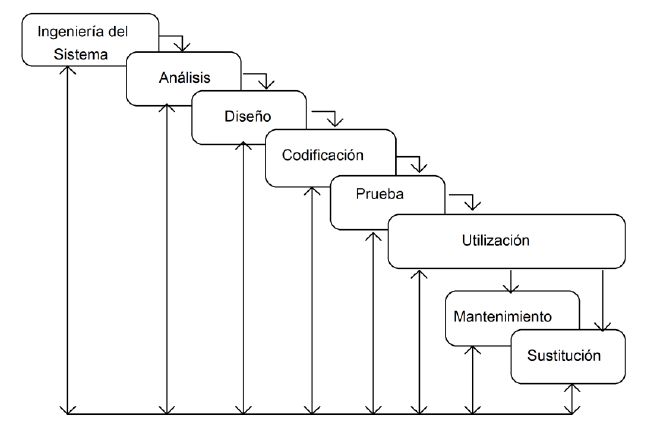
\includegraphics[width=0.7\linewidth]{Resources/cicloCascada}
  \caption{Etapas del ciclo de vida en cascada.}
  \label{fig:procesoCascada}
\end{figure}
 El ciclo de vida en cascada exige un enfoque sistemático y \textbf{secuencial} del desarrollo de software. Se dice que el modelo en cascada está guiado por documentos, ya que \textbf{nunca empieza la siguiente fase antes de que presente el documento de la anterior} (Tabla \ref{tab:cascadaDocumentos}).\\
 
\begin{table}[H]
\centering
\resizebox{\textwidth}{!}{%
\begin{tabular}{|l|l|}
\hline
\multicolumn{1}{|c|}{\textbf{Proceso}} & \multicolumn{1}{c|}{\textbf{Documentos Producidos}} \\ \hline
Especificaciones del sistema. & Especificación funcional. Arquitectura del sistema \\ \hline
Análisis de requisitos & Documento de requisitos \\ \hline
Diseño de la arquitectura del software & Especificación de la arquitectura \\ \hline
Diseño de interfaces & Especificación del diseño \\ \hline
Codificación & Código de programa \\ \hline
Prueba de unidades & Informe de pruebas de unidad \\ \hline
Prueba de módulos & Informe de pruebas de módulo \\ \hline
Prueba de integración & Informe de prueba de integración y manual de usuario final \\ \hline
Prueba del sistema & Informe de prueba del sistema \\ \hline
Prueba de aceptación & Sistema final más la documentación \\ \hline
\end{tabular}%
}
  \caption{Ejemplo de documentos producidos en un ciclo de vida en cascada. \textit{No tiene que tener exactamente las mismas fases que el ciclo en cascada por defecto.}}
  \label{tab:cascadaDocumentos}
\end{table}
 
 \subsection{Fases}
 \begin{enumerate}
 
     \item \textbf{Ingeniería y análisis del sistema}: Define las interrelaciones del software con otros elementos del sistema más complejo en el que esté englobado.
     
     \item \textbf{Análisis de requisitos del software}: Análisis detallado de los componentes del software incluyendo \textbf{datos} a manejar, \textbf{funciones} a desarrollar e \textbf{interfaces}.
     
     \item \textbf{Diseño}: \textbf{Estructura} de los datos, funciones, interfaces y aplicaciones.
     
     \item \textbf{Codificación}: Traducción del diseño a un formato que sea legible para la máquina. Produciendo un programa ejecutable.
     
     
     \item \textbf{Prueba}.
     
     \item \textbf{Utilización}.
     \item \textbf{Mantenimiento}.
     
     \begin{itemize}
         \item Errores latentes detectados por el cliente.
         \item Cambios en alguno de los componentes informáticos.
         \item Modificaciones funcionales requeridas por el cliente.
     \end{itemize}
 \end{enumerate}
 
 \subsection{Aportaciones}
 \begin{itemize}
    \item Es el más simple, conocido y fácil de usar.
    \item Los procesos definidos se \textbf{formalizan} en normas, \textit{sabes lo que tienes que hacer en cada momento}.
    \item Permite generar software eficiente, en el tiempo establecido en tiempo y forma (\textbf{funciona}).
    \item Al final de cada fase los interesados pueden comprobar el estado del proyecto.
 \end{itemize}
 
 \subsection{Problemas}
 \begin{itemize}
     \item En realidad el ciclo de vida \textbf{NO es secuencial}, ya que el \textbf{mantenimiento} y problemas con el proyecto exigen \textbf{volver atrás} a la parte donde se produjo el fallo. % 
     \item No siempre se pueden establecer los requisitos desde el primer momento. 
     \item Hasta que se llega a la fase final, no se dispone de una versión operativa del programa. 
     \item Los errores se detectan al final del proyecto, acentuando las pérdidas producidas por los fallos no detectados cometidos en fases anteriores.
 \end{itemize}
 
 \section{Ciclo de vida incremental} % Aquí la tipa se hecho un lío tremendo. Estaba todo mal.
% foto de incrementos
\begin{figure}[H]
  \centering
  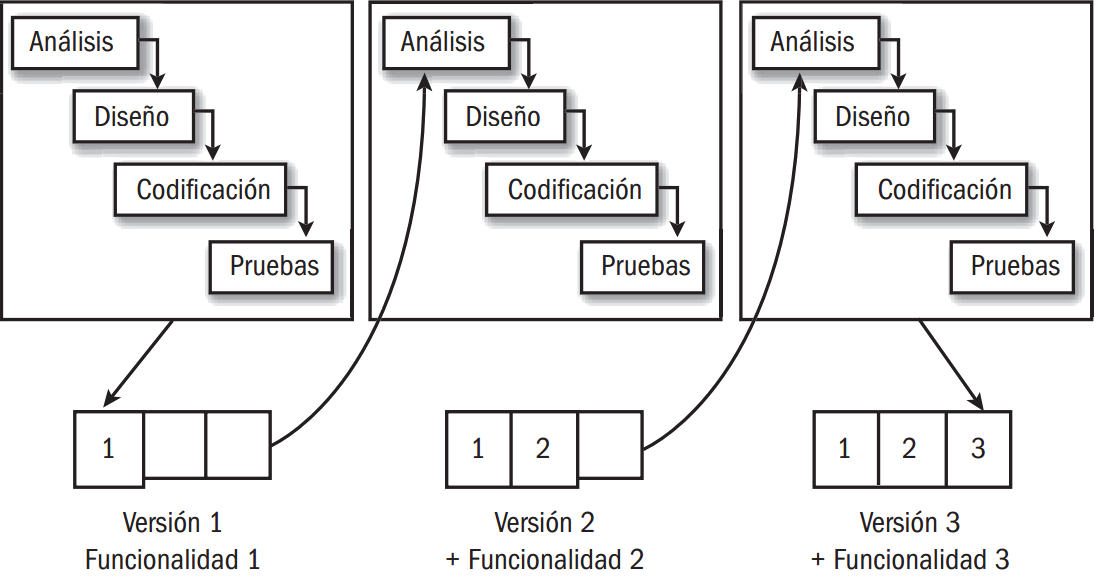
\includegraphics[width=0.7\linewidth]{Resources/cicloIncremental.png}
  \caption{Etapas del ciclo de vida incremental.}
  \label{fig:procesoIncremental}
\end{figure}

Surge como una \textbf{mejora del modelo en cascada} para paliar el problema de la \uline{detección de errores} y \uline{gestionar mejor los riesgos}.\\\\
Comenzamos como en cascada hasta la fase de diseño, completando solo el diseño preliminar. A partir de ahí separamos el proyecto en objetivos mas pequeños, que son \textbf{partes} del código \textbf{completas} y \textbf{funcionales} por sí mismas.\\\\
Para \textbf{cada incremento} realizamos las fases correspondientes de \textbf{diseño, codificación y explotación y mantenimiento}\footnote{A diferencia del resto de los mortales, Rabenso considera que el análisis no forma parte de los incrementos.}, obteniendo feedback.

\subsection{Ventajas}
%Tenemos por ahí el documento que hicimos de esto?
Soluciona parte de los problemas del modelo en cascada, mejorando la \textbf{comunicación con el cliente} y la \textbf{detección de errores} a tiempo.\\
Además, favorece la \textbf{modulación del software} al no pensarse como una unidad sino como la interacción de resultados sucesivos.\\

\subsection{Desventajas}
La parte de requisitos no se encuentra en la fase interactiva y por lo tanto tiene los problemas de cascada: es \textbf{difícil ver si los requisitos son válidos} y los \textbf{errores se detectan tarde}.





 \section{Construcción de prototipos}
 %Foto de ciclo prototipos
 \begin{figure}[H]
  \centering
  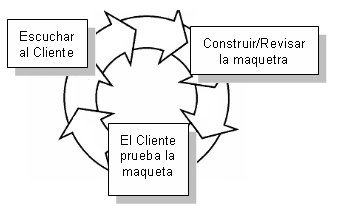
\includegraphics[width=0.7\linewidth]{Resources/construccionPrototipos.png}
  \caption{Etapas del paradigma de la construcción de prototipos.}
  \label{fig:construccionPrototipos}
\end{figure}

Consiste en la realización interactiva de prototipos hasta alcanzar un estado en el que los \textbf{requisitos} del sistema están \textbf{claros}, pasando entonces a desarrollar en cascada.\\


\subsection{Ventajas}

\begin{itemize}
    \item Muchas veces gran parte del \textbf{trabajo realizado} en los prototipos es \textbf{reutilizable}.
    \item En \textbf{proyectos con un nivel alto de incertidumbre}, donde los requisitos no están nada claros en primera instancia este ciclo provee un \textbf{método para obtener los requisitos de forma fiable} a través del feedback del usuario.
    \item Los prototipos permiten analizar \textbf{alternativas y viabilidades}. Refinando el resultado final o abortándolo antes de invertir demasiado dinero en el mismo.
\end{itemize}

\subsection{Problemas}
\begin{itemize}
   \item Es \textbf{posible que nunca se llegue a la fase de construcción}, lo cual da lugar a los problemas característicos de un software construido sin seguir procesos de ingeniería.
   \item Hay \textbf{mucha interacción con el cliente}, lo cual puede suponer un problema dependiendo de la predisposición del mismo a ver prototipos continuamente.
   \item Es imposible una \textbf{predicción de costes} fiable.
\end{itemize}



% Esto no recuerdo haberlo visto con Triñares. A mi me suena verlo muy de pasada
% Quizás lo que habría que hacer con esto es resumirlo en 10 líneas o menos.
\section{Técnicas de cuarta generación}
% yo creo que llega
% Sobra. Como mucho taboada pone una pregunta diciendo "son las técnicas de cuarta generación un desperdicio" o algo así.
%dejalo así Que son? y porque son mierda? no necesitas mas
Son un conjunto diverso de técnicas que permiten la generación de parte del código y la documentación; como el acceso a base de datos, interfaces gráficas e informes.\\\\
El mayor problema de estas técnicas es que el código que generan suele ser ineficiente y de menor calidad, requiriendo revisión y aumentando los costes de mantenimiento. Además no son fáciles de usar.\\\\ 
Sin embargo, a pesar de que no llegaron a conseguir los resultados esperados, reducen el tiempo y se utilizan sobre todo en software de gestión.


\section{Modelo en espiral}

%foto
 \begin{figure}[H]
  \centering
  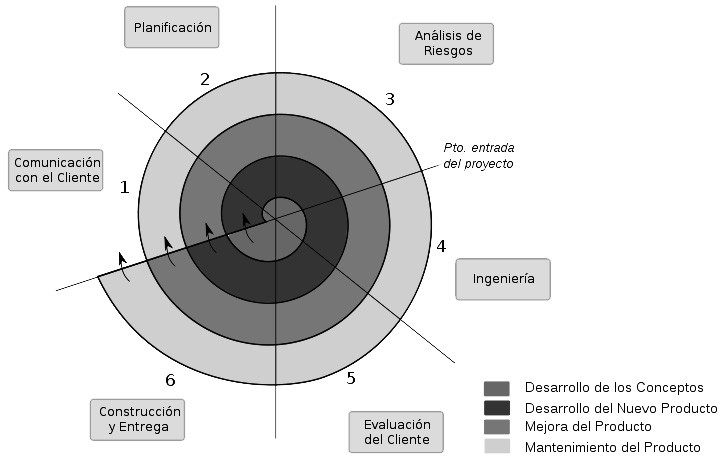
\includegraphics[width=0.7\linewidth]{Resources/modeloEspiral.jpg}
  \caption{Etapas del modelo en espiral.}
  \label{fig:modeloEspiral}
\end{figure}

Es un \textbf{modelo iterativo que combina las principales ventajas del modelo de ciclo de vida en cascada y el modelo de construcción de prototipos}. Del modelo en cascada sacamos la entrega de código ejecutable con funcionalidades válidas, estas entregas ahora son prototipos de la calidad requerida para cada fase habiendo pasado por fases previas de diseño.\\

    %Imagen del análisis de riesgos. La del magerit? trap 35 eso no es análisis, eso es administración del riesgo. Pero correcto
\subsection{Análisis de riesgos}
Este modelo incorpora, el análisis de riesgos basado en la identificación de amenazas a activos y el establecimiento de soluciones a esas amenazas (Administración de riesgos, Figura \ref{fig:administracionRiesgo}). Debemos pues:
\begin{enumerate}
   \item \textbf{Identificar los riesgos} Se identifican los activos, las amenazas y los riesgos potenciales (estimación del grado de exposición a que una amenaza se materialice en un activo). %tal cual los traparabas
   
   \item \textbf{Análisis de riesgos}: Estimación de la magnitud de los riesgos, obteniendo una lista de priorizanción de riesgos. 
   
   \item \textbf{Planificación de riesgos}: 
   Establecimiento de la estrategia adoptada contra el riesgo, pudiendo elegir entre:
   \begin{itemize}
      \item Estrategias de prevención.
      \item Estrategias de minimización.
      \item Planes de contingencia.
      % TODO aqui no falta transpaso, traspasar el riegos a otra empresa que lo gestione por ti?
   \end{itemize}
   \item \textbf{Gestión de riesgos}: Supervisar el desarrollo del proyecto, de forma que se detecten los riesgos tan pronto como aparezcan.
\end{enumerate}

\begin{figure}[H]
  \centering
  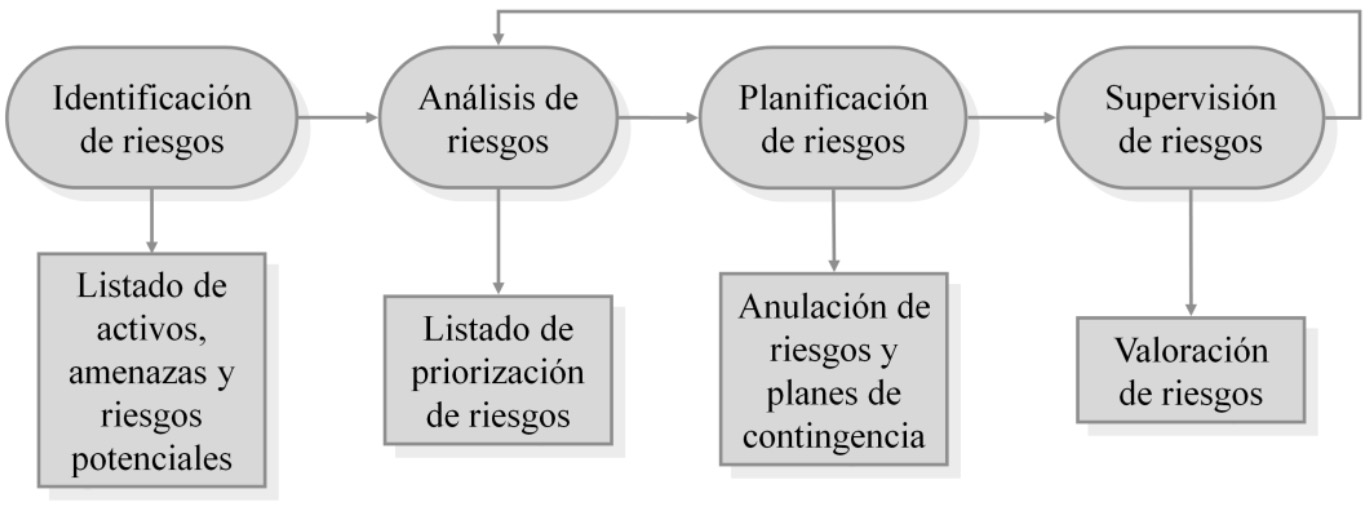
\includegraphics[width=0.7\linewidth]{Resources/administracionRiesgo.jpg}
  \caption{Administración del riesgos.}
  \label{fig:administracionRiesgo}
\end{figure}

% Esto que quieres hacer, un nuevo subsection? zumbale. Las imágenes han sido todas cambiadas a blanco y negro, mejorado el contraste para la hora de imprimir y limpiado si tenían manchas porque rabenso no sabe escanear.

\subsection{Descripción del modelo}
El modelo en espiral define 4 tipos de actividades de las que consta un ciclo:
\begin{enumerate}
   \item \textbf{Definición de objetivos}.
   \item \textbf{Análisis de riesgos}.
   \item \textbf{Desarrollo y validación}.
   \item \textbf{Revisión y planificación}: En ella se decide si se continúa con el proyecto o no, y se realizan planes para el siguiente ciclo.
\end{enumerate}



\subsection{Ventajas}% deducir, no las dice explícitamente
\begin{itemize}
   \item Entrega de prototipos con la calidad requerida para cada fase de código ejecutable con funcionalidades básicas válidas.
   \item Incorporación del análisis de riesgos.
\end{itemize}

\subsection{Desventajas}
\begin{itemize}
   \item Es difícil de adaptar a un contrato, aunque se puede utilizar el modelo de contrato por iteración.
   \item Requiere habilidad en la gestión de riesgos.
   \item Un riesgo no detectado a tiempo es similar a un requisito no detectado a tiempo. %no se porqué eso es un incomveniente pero rabo
   \item Requiere muchos recursos para su control, y es difícil convencer al cliente de que lo estás controlando.
\end{itemize}

\section{Metodologías ágiles}
% RRHH  meets RABENSO

%Sorprendente estos dos párrafos están bien.
El desarrollo ágil defiende la renuncia a utilizar modelos perfectos, se basa únicamente en que sean lo suficientemente buenos. Tratan de \textbf{centrar los esfuerzos en presentar un incremento software ejecutable}, restando importancia a los productos de trabajo intermedio.
\\\\
Los \textbf{incrementos son valorados por el cliente}, que entra de forma efectiva en el proceso desarrollo del software y ofrece la necesaria realimentación al equipo de desarrollo.
\\\\
Las metodologías pesadas se enfrentan a las limitaciones de las personas que intervienen en los procesos, mientras que las metodologías ligeras adoptan un \textbf{enfoque de tolerancia donde el modelo se adapta al equipo} y no a la inversa.

\subsection{Equipo ideal para las metodologías ágiles}
Debe buscarse un equipo con los siguientes rasgos (que suenan a algo que diría un \textit{young business entrepreneur}):
\begin{itemize}
   \item \textbf{Competencia} sobre el proceso.
   \item \textbf{Enfoque común}, la meta es la entrega rápida.
   \item \textbf{Colaboración} entre stakeholders.
   \item \textbf{Habilidad para la toma de decisiones}, necesaria para una entrega rápida.
   \item \textbf{Capacidad de resolución de problemas confusos} ante la no concreción de requisitos.
   \item \textbf{Confianza y respeto mutuo}. %NO cuernos joder
   \item \textbf{Capacidad de autoorganización}. %Ala
\end{itemize}

\paragraph{Principios para alcanzar la agilidad}

\begin{enumerate}
    \item La mayor prioridad es \textbf{satisfacer al cliente} mediante la entrega temprana y continua de software valioso.
    \item Bienvenidos los \textbf{requisitos cambiantes}, incluso en fases tardías del desarrollo.
    \item \textbf{Entregar con frecuencia} software en funcionamiento.
    \item La \textbf{gente de negocios} y los \textbf{desarrolladores} deben \textbf{trabajar juntos} a diario. % Reunión Reunión Reunión! Reunión Reunión Reunión!
    \item Construir \textbf{proyectos alrededor de individuos motivados}. Darles el ambiente y soporte necesario que necesitan, y confiar en ellos para obtener el trabajo realizado. % MOTÍVATE
    \item El método más eficiente y efectivo para transmitir información es la \textbf{conversación cara a cara}.
    \item \textbf{El software en funcionamiento es la medida primaria de progreso}.
    \item Los procesos ágiles promueven el \textbf{desarrollo sostenible}. %Porque lo dices tú
    \item La atención continua a la excelencia técnica y al buen diseño mejora la agilidad.
    \item La simplicidad es esencial. %Por eso ponemos 12 principios.
    \item Las mejores arquitecturas, los mejores requisitos y los mejores diseños emergen de \textbf{equipos autoorganizados}.
    \item A intervalos regulares el \textbf{equipo refleja} la forma en que se puede \textbf{volver más efectivo}.
\end{enumerate}
%Puedo poner algo en lo de los equipos?

\subsection{Modelado ágil}
A \textbf{alto nivel} es una \textbf{colección de buenas prácticas}, entrando \textbf{en detalle} es una \textbf{colección de valores}, principios y practicas. Puede ser tomado más como una filosofía que como una metodología: 
\begin{itemize}
   \item Modelar con un propósito.
   \item Usar múltiples modelos.
   \item Viajar ligero: Conservar sólo los modelos que proporcionarán valor a largo plazo.
   \item El contenido es más importante que la representación.
   \item Conocer los modelos y herramientas con que se crean.
   \item Adaptar al equipo ágil.
\end{itemize}

\subsection{Programación extrema}
 \begin{figure}[H]
  \centering
  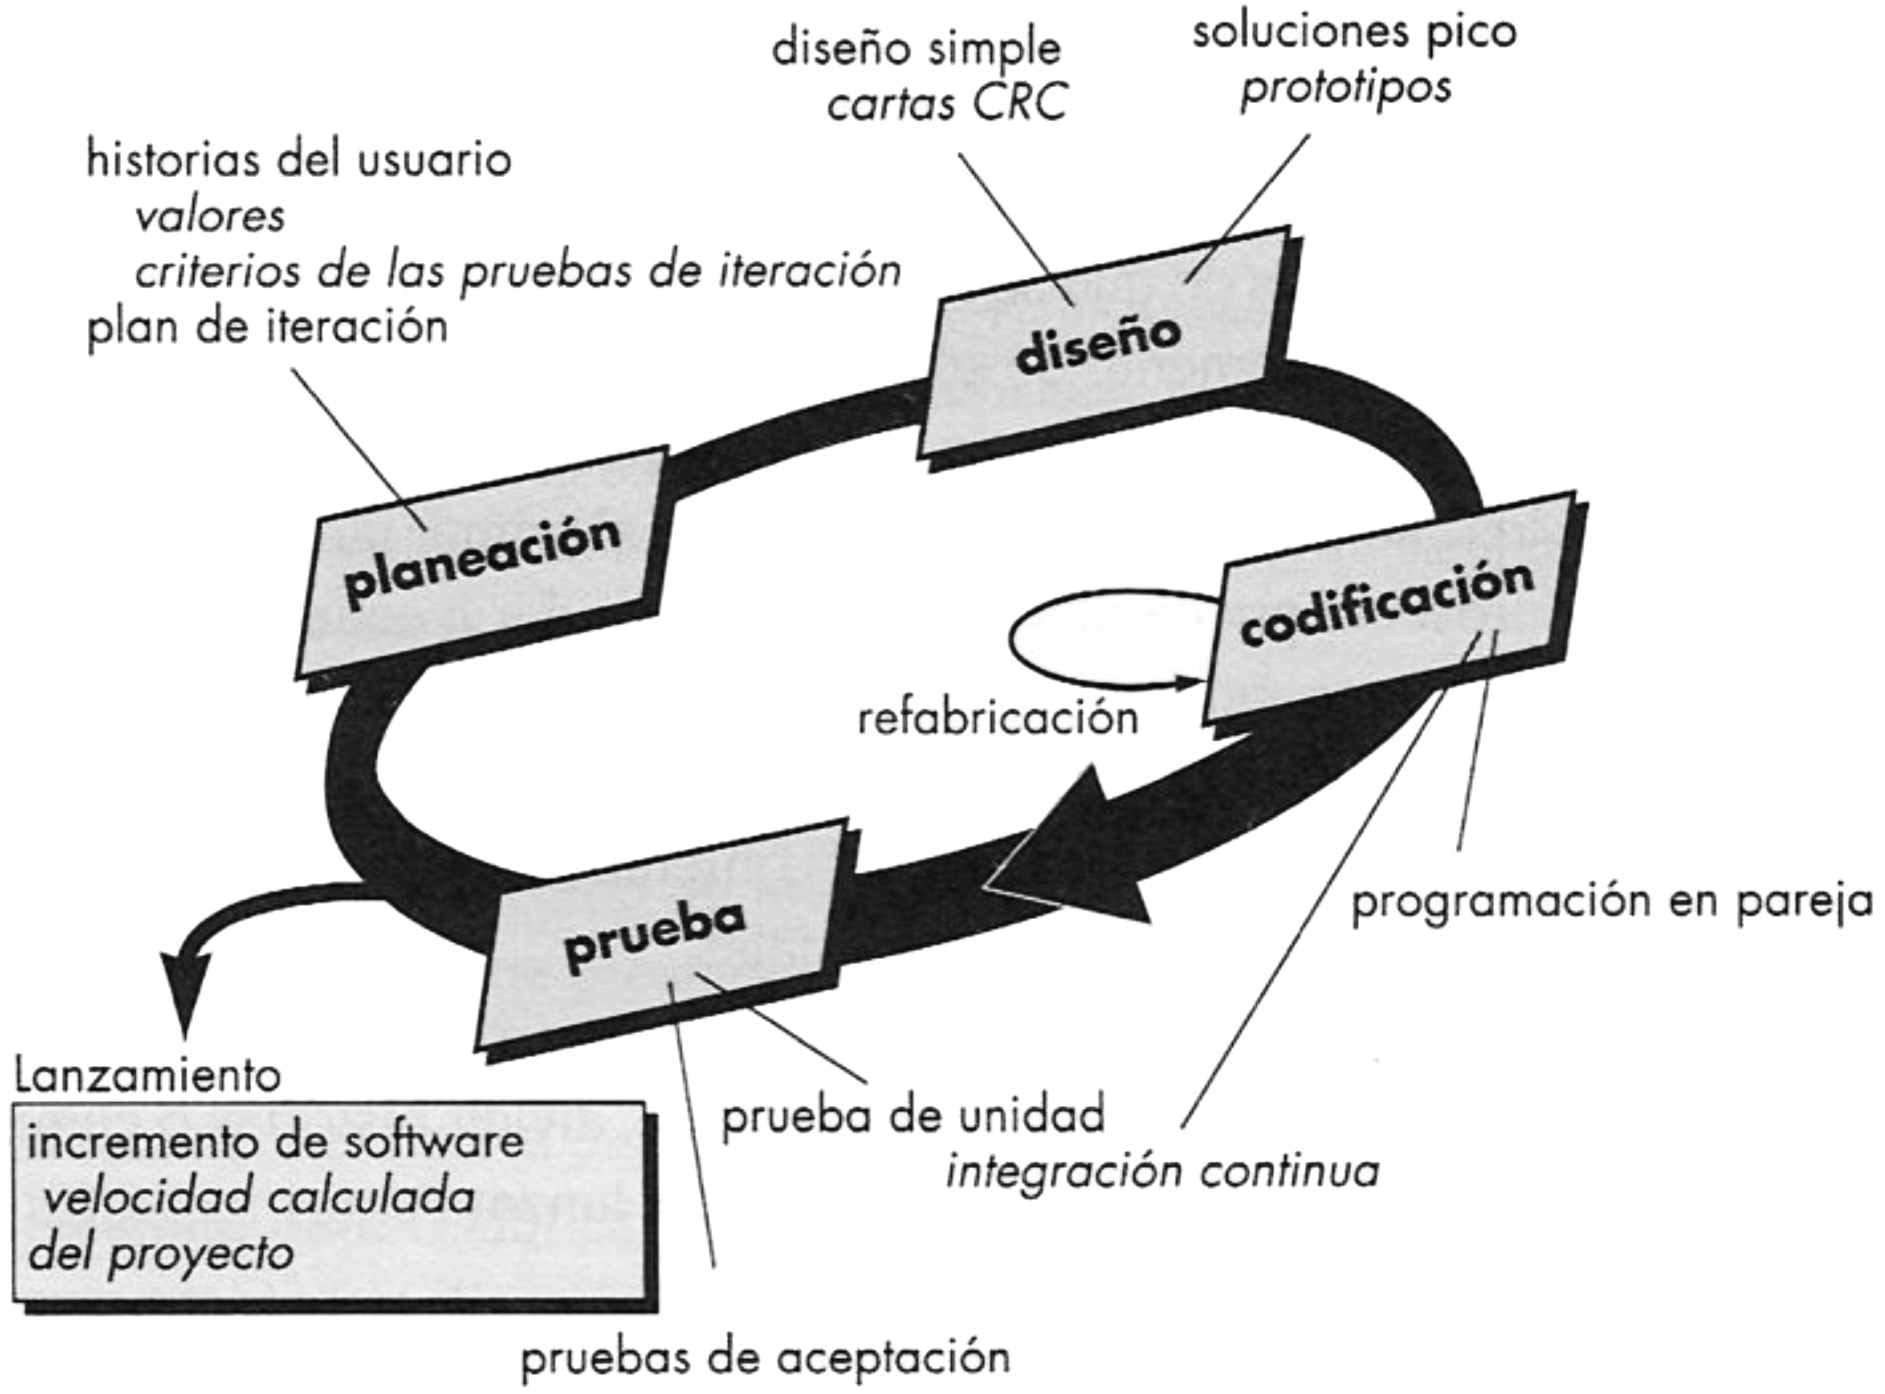
\includegraphics[width=0.7\linewidth]{Resources/programacionExtrema.jpg}
  \caption{Etapas de la programación extrema.}
  \label{fig:programacionExtrema}
\end{figure}
% Venga lo dejo
\textbf{Utiliza un enfoque orientado a objetos}: Abarca un conjunto de reglas que ocurren en el contexto de las siguientes actividades:
\begin{enumerate}

    \item \textbf{Planificación}:
    \begin{itemize}

       \item \textbf{Creación de historias de usuario}: Utiliza historias de usuario para establecer los requisitos, a las que se el usuario asigna un valor de prioridad.
       \item \textbf{Estimación del tiempo de implementación}: Si es superior a 3 semanas se reescribe la historia.
       
       \item \textbf{Plan de construcción}: Los clientes y el equipo se reúnen para decidir qué historias hay en el siguiente incremento, priorizando de la siguiente forma:
       \begin{itemize}
          \item Todas las historias serán implementadas de un modo inmediato.
          \item Las historias con \textbf{valor más alto} se moverán en el programa y se implementarán al \textbf{principio}.
          \item Las historias de \textbf{mayor riesgo} se moverán en el programa y se implementarán al \textbf{principio}.
       \end{itemize}
       Después de que se haya entregado el primer lanzamiento, se calcula la \textbf{velocidad del proyecto}, que es el número de historias del cliente implementadas en el primer lanzamiento. 
       
       La velocidad se puede usar para ayudar a estimar fechas de entrega o determinar si se ha hecho un compromiso excesivo en algunas historias, en cuyo caso se modifica el contenido de los lanzamientos o se cambian las fechas de entrega.
          
    \end{itemize}
    
    
   \item \textbf{Diseño}: Sigue el principio KISS (\textit{Keep It Simple, Stupid}) y se apoya en: 
   % https://en.wikipedia.org/wiki/KISS_principle El stupid es importante. Porque somos estúpidos y debemos recordarlo.
   \begin{itemize} %Mejor así.
      \item \textbf{Tarjetas CRC} (Colaborador--Responsabilidad--Clase). 
      \item \textbf{Prototipado}: Para la resolución de problemas difíciles, se recomienda construir prototipos.
      \item \textbf{Prefabricación}: Nos apoyamos en mejorar la estructura interna del software sin que se altere el comportamiento externo.
      \item \textbf{Diseño como artefacto}: Se permite la modificación del diseño durante la construcción.
   \end{itemize}

   \item \textbf{Codificación}: Se prefiere crear las \textbf{pruebas antes que el código} de las clases.
   
   \item \textbf{Pruebas}: Se distinguen:
   \begin{itemize}
      \item \textbf{De unidad}: realizadas a diario y a ser posible, de forma automatizada para evitar que los problemas se vuelvan enormes.
      \item \textbf{De aceptación}: especificadas por el cliente, enfocadas a características generales y de funcionalidad del sistema que el cliente puede revisar. %Lo de que son elementos visibles y revisables por el cliente es redundante.
   \end{itemize}
% Los temas van a peor el 4, 5 y 6 están muy intratablesTM.
\end{enumerate}
